\documentclass[11pt,letterpaper]{article}
\usepackage[latin1]{inputenc}
\usepackage{amsmath,amsfonts,amssymb,bm,geometry,url}
\usepackage{subfigure,graphicx,algorithm,amsmath,algpseudocode}
\usepackage{color, framed}

\newcommand{\todo}[1]{\textcolor{red}{TODO: #1}}

\oddsidemargin = 0in
\evensidemargin = 0in
\topmargin = -0.5in
\headheight = 0in
\textwidth = 6.5in
\textheight = 8.75in

\title{CS 284: Problem Set 4 \\ Sampling-Based Planning}
\author{100 points possible. \textbf{Due Friday, April 1st}}
\date{}
\begin{document}
\maketitle

\begin{framed}
\noindent Submission instructions: Please submit your solutions to \textbf{Canvas} as a .zip file containing 1) a PDF (preferably \LaTeX-formatted) and 2) your source code for all problems.
\end{framed}

\begin{enumerate}

\item \textbf{Vanilla RRT [30 points]} In this problem, you will implement the Rapidly Exploring Random Tree (RRT) algorithm. For easy visualization, we will consider a two dimensional example. However, it will be relatively straightforward to extend your code to handle higher dimensional environments.


\begin{enumerate}
\item The most computationally expensive portion of the algorithm is typically the collision checker. Write code that will take a set of points determine if a given set of points $x_i \in \mathcal{X}$ are in the convex hull of another set of points $y_j \in \mathcal{Y}$. The output of your code should be a row vector of boolean variables whose $i$th element is {\tt true} if and only if $x_i$ is not in the convex hull.

Hint: The Matlab functions convhull and inpolygon may be useful to you here (but of course, you don't have to use them). Make sure to check your code by making plots a few times before continuing to part (b).

	\begin{figure}[th]
		\centering
		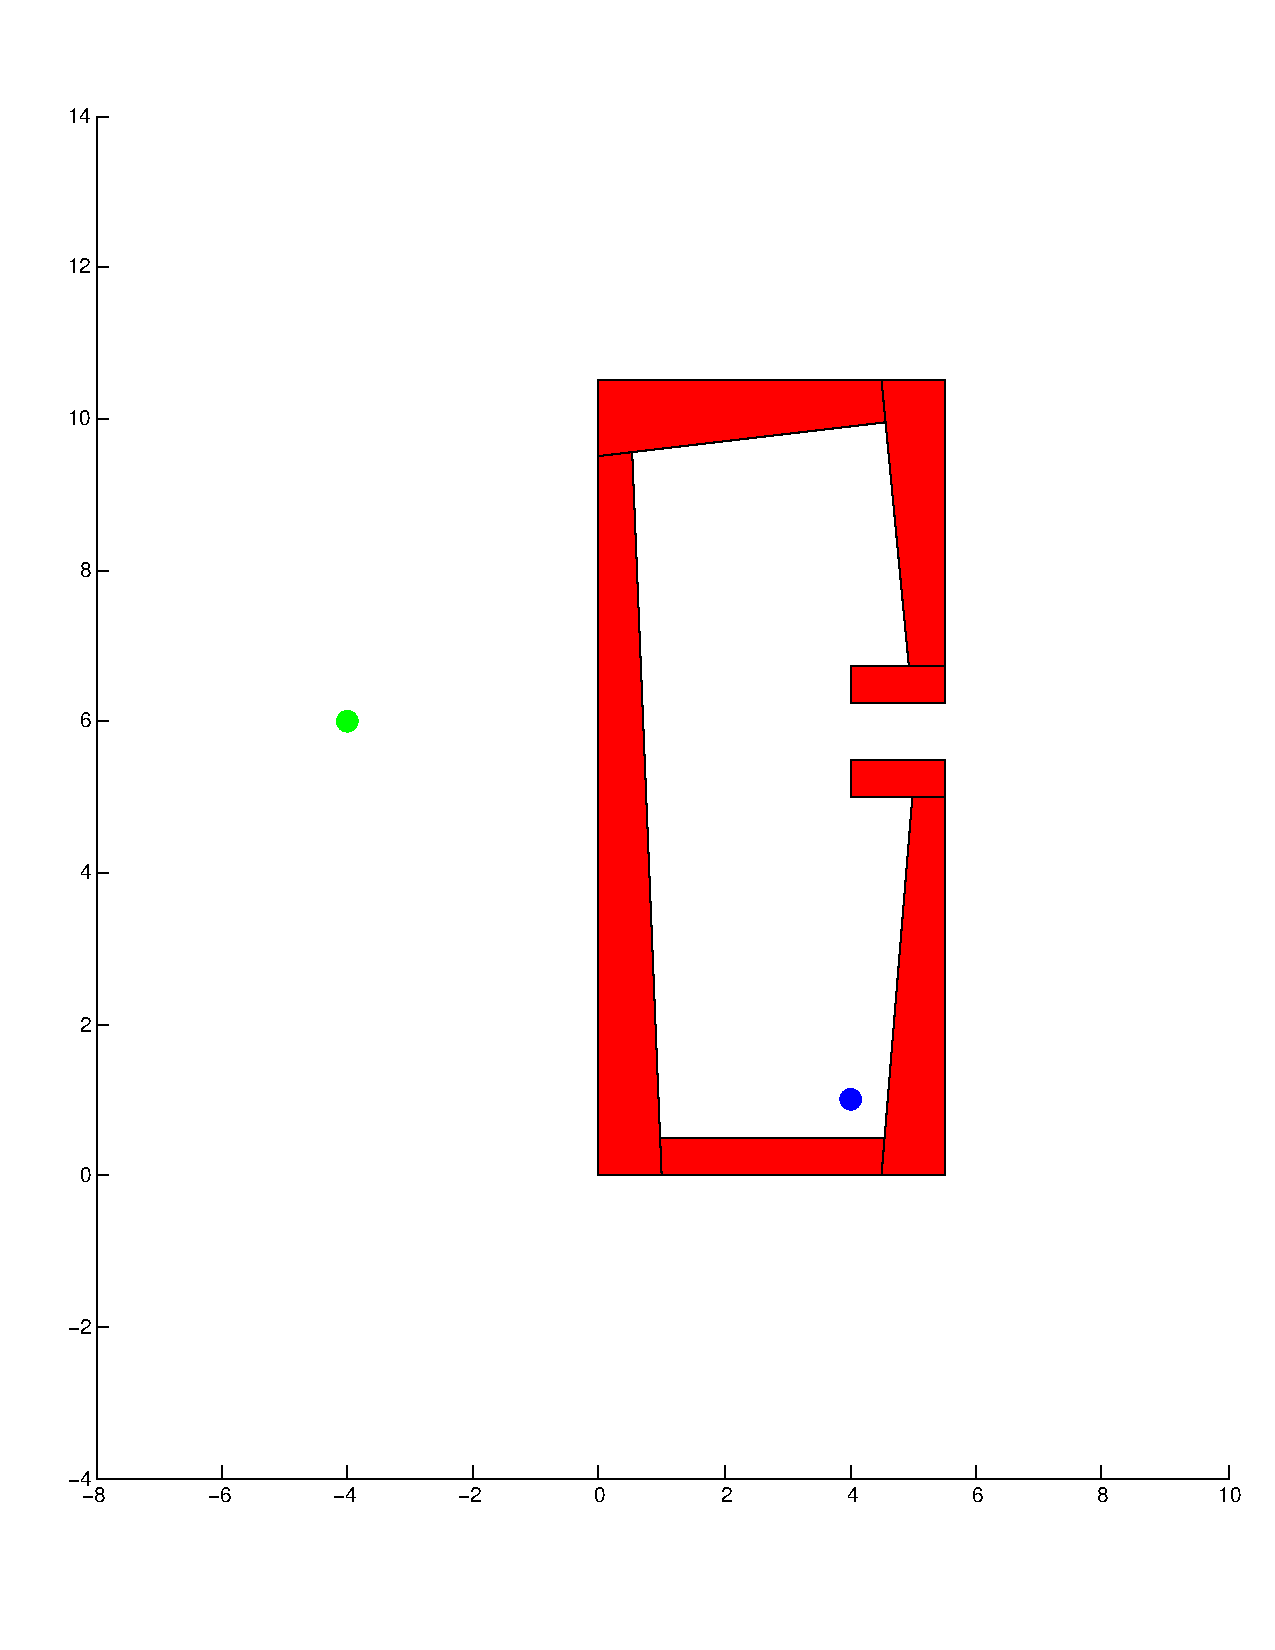
\includegraphics[width=3.0in]{bugtrap}
		\caption{A simple ``bugtrap'' environment.}\label{fig:bugtrap}
	\end{figure}

\item Next, you will implement the entire RRT algorithm and test it out on a ``bug trap'' environment (shown in Figure~\ref{fig:bugtrap}). This kind of environment is typically quite challenging for motion planning algorithms since it requires discovering and navigating through a narrow passage in order to get out of the ``trap.'' However, hopefully you'll see that the RRT algorithm is able to do this with relative ease.


Fill in the missing portions of the provided code. Run your code 10 times and report the number of nodes created for each run. 
\end{enumerate}

\item \textbf{Bi-Directional RRT [20 points]} For the same bug trap problem above (in a separate file called {\tt bugtrap-twotree.m}, implement a bi-directional RRT (see \url{http://planning.cs.uiuc.edu/node237.html}) to solve it. Try to demonstrate superior median performance compared to the standard RRT algorithm you implemented in Problem 1.  Run your code 10 times and report the number of nodes created for each run. 

\item \textbf{RRT-Pendulum [50 points]} In this problem, you will consider extensions of the RRT algorithm that allow us to handle dynamic constraints. In particular, we will consider the swing-up problem for a torque-limited pendulum as our test-bed. The dynamics for the pendulum will be:

\[ \ddot{\theta} = u - g \sin (\theta) -b \dot{\theta}, \]
where $g=9.81$, $b=0.1$, and $u=\in [-5,5]$. 

The stub code provided in {\tt pend.m} is similar to the bug trap problem---the only differences will be in the way we find the closest vertex in our existing tree (given a new sample) and the way we extend the tree. In particular, the extension operation must satisfy the dynamic constraints of the system. Please take a quick look at the code to make sure you understand the basic structure.

\begin{enumerate}

\item  As a first step, you will consider the Euclidean metric to determine the closest vertex to a new sample. One thing that you need to be careful about is that $\theta$ wraps around. In particular, $\theta$ will lie between $-\pi/2$ and $3\pi/2$. Thus,  the angles $-\pi/2$ and $3\pi/2$ are in fact the same. Given this representation, what is the Euclidean distance between the states $[-2;3]$ and $[4;1]$?

\item Next, you will implement the RRT algorithm using the Euclidean metric as our distance function. In order to do this, you will need to fill in the missing parts of the code by implementing the following:

\begin{itemize}
\item Implement the function {\tt closestVertexEuclidean(rrt\_verts,xy)} that takes in a $2\times K$ vector consisting of the current vertices of the RRT, along with a state {\tt xy} and returns the vertex in the tree that is closest to {\tt xy}.
 
\item Implement the function {\tt extendEuclidean(closest\_vert,xy)} that will perform the extend operation in the following manner. Discretize the range of control inputs in $[-5,5]$ (around 20 discrete samples should be sufficient) and choose the input $u_0$ that will result in the system moving the most in the direction of the sample point {\tt xy} when started from the state {\tt closest\_vert} (there are many ways to make this choice). Simulate the system (using ode45 for example) for a small time interval (no more than 0.1 seconds) using this constant control input to obtain {\tt new\_vert}. Be sure to correctly wrap the angle coordinate. Also make sure to implement the input saturations in your simulation.

	Run your code a few times. You should find that it succeeds. Does the performance seem reliable and efficient? State your observations. 
\end{itemize}

\item Next you will now consider an alternative based on LQR that should improve the performance of your code from part (b).

Given a nominal state $x_0$ and control input $u_0$, we can linearize the dynamics $\dot{x} = f(x,u)$ about this point:

\[ \dot{x} \approx f(x_0,u_0) + \frac{\partial f(x_0,u_0)}{\partial x} (x-x_0)+ \frac{\partial f(x_0,u_0)}{\partial u} (u-u_0)  \]

We can then define a change of variables $\bar{x} = x-x_0$ and $\bar{u} = u-u_0$. Then we have:

\[ \dot{\bar{x}} =  A\bar{x} + B\bar{u}\]
where $A$ and $B$ are the partial derivatives of $f$ with respect to $x$ and $u$, respectively. 

Given a quadratic cost function defined by state and action cost matrices $Q$ and $R$, we can solve a LQR problem ({\tt [K,S] = lqr(A,B,Q,R)} in Matlab). Then the locally optimal policy is given by $u^*(\bar{x})=-K\bar{x} + u_0$. The metric we will use to determine how close a point $x$ is to $x_0$ is then given by the optimal cost-to-go, $(x-x_0)^T S (x-x_0)$. 

Let $Q=I$, $R=0.1$, $x_0=[\pi-0.1;2.0]$, and $u_0=0$. What is the ``distance''---evaluated by the metric just described---between $x_0$ and $x=[\pi+0.25,3.0]$?

\item Next, you will use the LQR metric from (c) in the RRT algorithm. In order to do this, you will need to implement the following:

\begin{itemize}
	\item Implement the function {\tt closestVertexLQR(rrt\_verts,xy)} that takes in a $2\times M$ vector consisting of the current vertices of the RRT, along with a state {\tt xy} and returns the vertex in the tree that is closest to {\tt xy} (as measured by the LQR metric), along with the gain matrix of the LQR policy. Make sure to handle the wrapping of the angle variable correctly.

\item Implement the function {\tt extendLQR(closest\_vert,xy,K)} that will perform the extend operation by applying the LQR policy starting from the state {\tt closest\_vert} for a short time interval (no more than 0.1 seconds). Here, you should use $x_0=xy$ and  $u_0=0$ to find the LQR policy. You can use ode45 again for the integration. Also make sure to implement the input saturations in your simulation.
 
\item Modify your code to output the path from start to goal found by the RRT. This should be a $L\times 2$ array. Given that this array is called {\tt xpath}, you can use the code provided here to visualize the path using the {\tt PendulumVisualizer} in the {\tt examples/Pendulum} folder in drake (you'll need to be in this folder to run this). 
	
Once you are satisfied that the path has been correctly obtained, plot the resulting path. 

\end{itemize}

\end{enumerate}

\end{enumerate}
\end{document}


